\subsection{Estructura de la red telefónica}
Se trata de un sistema con bloqueo, se puede variar con sistemas adicionales como el buzón de voz o similares a un sistema con espera. Cuando era analógica la red telefónica se trataba de un sistema de conmutación de circuitos.\\
Las centrales de conmutaciónse basan en la idea de conmutación multietapa, con esto se evita el tener un cable por destino. La estructura jerarquica de la red telefónica está descrita a continuación:
\begin{itemize}
\item Un par de abonado entre cada cliente y la central local. [CL]
\item Central primaria enlaza 2 o más centrales locales. [CP]
\item Bucle de abonado, del abonado a la central local.
\item Enlace troncal, los internos entre centrales, también llamados enlace final.
\item Central secundaria une dos o más centrales primarias. [CS]
\item Central terciaria y superiores enlazan dos o ás centrales de orden inferior. [CT]
\item Una ruta final está unicamente formada por enlaces finales.
\end{itemize}
\begin{figure}[H]
\centering
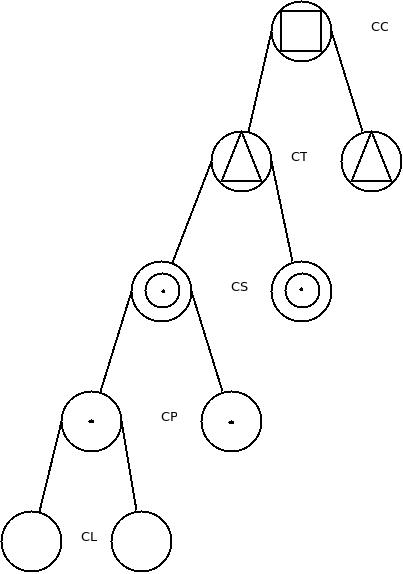
\includegraphics[width=0.9\textwidth]{Imagen/diajerartelefono.jpg}
\caption{Diagrama de la red jerárquica}
\label{diaRedTelefonica}
\end{figure}
A parte de la red jerarquica existe la red complementaria. Esta está formada por enlaces directos. Enlaces que unen centrales que no están unidas jerarquicamente.\\
\subsubsection{Encaminamiento en la estructura de la red telefónica}
\begin{enumerate}
\item Identificamos el arbol de destino. Está formado por todos los nodos jerarquicamente superiores al nodo de destino.
\item En cada nodo vemos si hay una sección directa que nos lleve al arbol de destino. No se pueden tomar 2 secciones directas en la misma ruta. Una sección directa nunca desbordará sobre otra sección directa, siempre desbordará sobre la sección final.
\item una vez en el arbol de destino desciendo jerarquicamente hasta el nodo destino.
\end{enumerate}
\begin{example}[Encaminamiento en la red telefónica]
\begin{figure}[H]
\centering
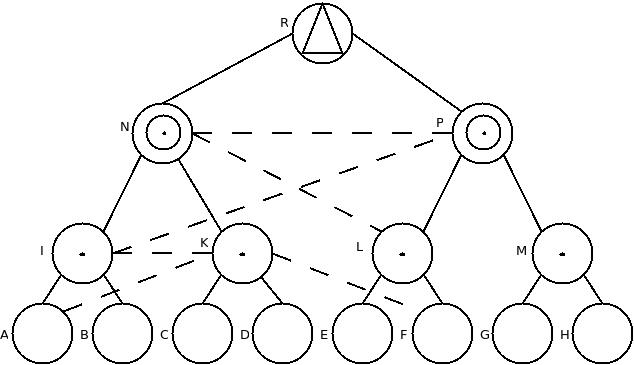
\includegraphics[width=0.9\textwidth]{Imagen/ejemploredtelefonica.jpg}
\label{}
\end{figure}
De la figura podemos sacar las siguientes rutas.\\
\begin{center}
\begin{tabular}{c c c c}
A$\to$C & AKC  		& A$\to$E 	& AIPLE 	\\
 		& AIKC 		&			& AINLE		\\
 		& AINKC		&			& AINRPLE	\\
E$\to$A & ELNIA  	& 		 	& 		 	\\
 		& ELPIA 	&			& 			\\
 		& ELPRNIA	&			& 			\\
\end{tabular}
\end{center}
Como se puede ver no todas las rutas son 100\% simétricas.
\end{example}
\subsubsection{Red inteligente}
Surge con la digitalización y a la vez que la Red Digital de Servicios Integrados (RDSI). Este sistema ofrece servicios de valor añadido.
\begin{figure}[H]
\centering
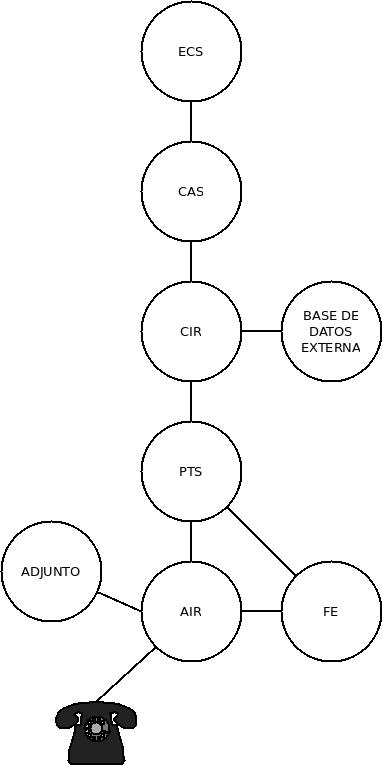
\includegraphics[width=0.5\textwidth]{Imagen/diaredinteligente.jpg}
\caption{Diagrama de la Red Inteligente}
\end{figure}
\begin{itemize}
\item Agencia de Inteligencia de Red [AIR]: Identifica si la llamada está destinada a la Red Inteligente. Solo hay una por Central Local.
\item Punto de Transferencia de Señalización [PTS]: Es un centro de intercambio entre las diferentes partes de la red.
\item Centro de Inteligencia de Red [CIR]: Es la parte más importante de la Red Inteligente ya que es el que reconoce los servicios y da las ordenes.
\item Adjunto: Es como el CIR pero se encuentra en la Central Local. De esta forma descarga las instancias superiores de la red.
\item Módulo de Funciones Especiales [FE]: Cumple varias funciones como la sintesis de voz o la captación de teclas marcadas.
\item Base de datos externa: Se trata de un conjunto de bases de datos que no se encuentran dentro del CIR, como la de tarjetas de crédito.
\item Centro de Administración de Servicios [CAS]: Lugar donde se administra y controla todos los servicios de la red. Este no tiene por que estar conectado a la red constantemente.
\item Entorno de Creación de Servicios [ECS]: Lugar donde se implementan los nuevos servicios. Este no tiene por que estar conectado a la red constantemente.
\end{itemize}
\subsubsection{Ejercicios}
\begin{exercise}[5]
La red telefónica de la figura tiene una probabilidad de pérdidas en las secciones finales del 1\% y una probabilidad de desbordamiento en las secciones directas del 10\% .
\begin{figure}[H]
\centering
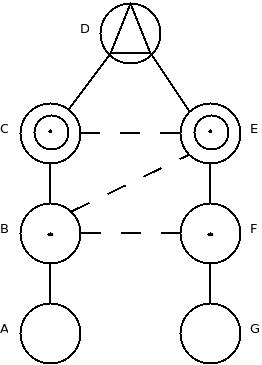
\includegraphics[width=0.5\textwidth]{Imagen/ejercicio5tema1.jpg}
\label{}
\end{figure}
La matriz de tráfico (simétrica) en Erlangs es la siguiente:
\begin{center}
\begin{tabular}{| c | c | c | c | c | c | c | c |}
\hline
   & A & B & C & D & E & F & G \\\hline
 A & - & 10 & 15 & 5 & 2 & 1 & 1 \\\hline
 B &   & - & 50 & 15 & 6 & 3 & 2 \\\hline
 C &   &   & - & 80 & 30 & 10 & 5 \\\hline
 D &   &   &   & - & 90 & 15 & 5 \\\hline
 E &   &   &   &   & - & 60 & 18 \\\hline
 F &   &   &   &   &   & - & 12 \\\hline
\end{tabular}
\end{center}
Se pide:\\
\textbf{1.} Indicar los caminos que comunican los nodos E y A.\\
\begin{center}
\begin{tabular}{c c c c}
E$\to$A & EBA  		& A$\to$E 	& ABE 	\\
 		& EDCBA		&			& ABCE	\\
 		& 			&			& ABCDE	\\
\end{tabular}
\end{center}
\textbf{2.} Calcular el tráfico ofrecido y cursado en la sección directa C$\to$E.\\
\begin{gather*}
TO_{C\to E}=TO_{CEpropio}+TO_{BEdesb}+TO_{BFdesb}+TO_{CF}+TO_{CG}=\\
30+0.8+0.7+10+5=46.5E\\
TO_{BE}=TO_{BEpropio}+TO_{AE}=8E\\
TO_{BEdesb}=TO_{BE}P_d=TO_{BE}0.1=0.8E\\
TO_{BF}=TO_{BFpropio}+TO_{BG}+TO_{AF}+TO_{AG}=7E\\
TO_{BFdesb}=TO_{BF}P_d=TO_{BF}0.1=0.7E\\
TC_{C\to E}=TO_{C\to E}(1-P_D)=41.85E
\end{gather*}
\textbf{3.} Considerando solo el tráfico saliente de A y sabiendo que la probabilidad de que la duración de la llamada sea superior a 5 minutos es de 0.08205, ¿cuál es la duración media de la llamada?\\
Se trata de un sistema con bloqueo M/M/c/c con $A_{oA}=34E=\frac{\lambda}{\mu}$.
\begin{gather*}
P(W>5min)=\int_{5}^{\infty}\mu e^{-\mu t}dt=-e^{-\mu t}\Big|_{5}^{\infty}=0.08205\\
\mu=0.5\sfrac{llamadas}{minuto}\to E(s)=2\sfrac{minutos}{llamada}
\end{gather*}
\textbf{4.} ¿Cuántos intentos de llamada se hacen en la hora cargada(HC)?\\
\begin{gather*}
A_{oA}=34E=\frac{\lambda}{\mu}\\
\mu=0.5\sfrac{llamadas}{minuto}\\
\lambda=34*0.5=17\sfrac{llamadas}{minuto}\\
\lambda_{HC}=17*60=1020\sfrac{llamadas}{hora}
\end{gather*}
\textbf{5.} Los registradores de la central A analizan las primeras cifras y encaminan las llamadas, pudiéndose modelar como un sistema M/M/c. Si el tiempo de ocupación de los registradores por cada llamada es de 6 segundos, ¿cuántos son necesarios para que la probabilidad de esperar más de 1 segundo sea de 0.008?\\
\begin{gather*}
E(s')=6\sfrac{segundos}{llamada}\to A'_o=\frac{\lambda}{\mu '}=1.7E\\
P(W_q>1s)=0.008=C(c,A'_o)e^-c\mu 'T(1-\rho)
\end{gather*}
Este apartado habrá que hacerlo por prueba y error hasta hallar el número de servidores necesarios para cumplir con las especificaciones. Se puede ver estas pruebas en la tabla:\\
\begin{center}
\begin{tabular}{c | c | c | c}
$C(c,A'_o)$ & c & $\rho$ & $P(W_q>1)$ \\\hline
0.7  & 2 & 0.85  & 0.6672 \\
0.1  & 4 & 0.425 & 0.0692 \\
0.008 & 6 & 0.283 & 0.00402
\end{tabular}
\end{center} 
De la tabla se puede observar que el número mínimo de registradores ha de ser 6.\\
\textbf{6.} ¿Cuál es el tiempo medio de espera en los registradores?\\
\[W_q=\frac{E(s)\rho}{1-\rho}=2.3682segundos\]
\end{exercise}
\begin{exercise}[6]
En un territorio de un país en vías de desarrollo, se ha decidido crear una nueva red telefónica digital. Para su planificación se han considerado los siguientes datos:
\begin{itemize}
\item Tras agrupar geográficamente los diferentes núcleos en entidades de población, resultando 83, se han obtenido 70 entidades  con 20000 habitantes, 10 con 60000, 2 con 1000000 y 1 (la capital) con 2000000
\item Se considera un grado inicial de penetración del servicio del 30\% (30 teléfonos por cada 100 habitantes). El incremento futuro de dicho porcentaje será absorbido por las correspondientes ampliaciones.
\item El tráfico total (entrante y saliente, excluyendo el local) por abonado se cifra en 20mE.
\item Se dispone de unidades locales de 6000 líneas.
\item Las centrales primarias tienen una capacidad para 3000E de tráfico total (entrante y saliente).
\item Existirá una central secundaria por cada 5 primarias y solo una central terciaria.
\item Sólo se establecen rutas finales, con una probabilidad de pérdida del 2\% (se puede aproximar la función de Erlang B por $B(A_o,c)=0.025\sfrac{A_o}{c}$.
\end{itemize}
Se desea conocer:\\
\textbf{1.} El número de unidades locales de conmutación necesarias.\\
\begin{gather*}
CL=(70\frac{20000}{6000}+10\frac{60000}{6000}+2\frac{1000000}{6000}+1\frac{2000000}{6000})30\%\\
CL=300\text{ centrales locales}
\end{gather*}
\textbf{2.} Los sistemas MIC de norma europea que permitirán la conexión de cada unidad local con su correspondiente primaria.\\
Cada unidad local genera $A_{oCL}=6000*0.02=120E$ con una probabilidad de pérdida del 2\% y utilizando la función Erlang B obtenemos:
\begin{gather*}
B(A_o,c)=0.025\sfrac{A_{oCL}}{c}=0.02\\
c=\frac{0.025A_{oCL}}{0.02}=150\text{ canales}\\
MIC=\frac{c}{30}=5\text{ sistemas MIC de norma europea}
\end{gather*}
\textbf{3.} El número de centrales primarias.\\
\[CP=\frac{300}{\frac{3000E}{6000*0.02E}}=12\text{ centrales primarias}\]
\textbf{4.} El número de centrales secundarias.\\
\[CS=\frac{12}{5}=2.4\to 3\text{ centrales secundarias}\]
\end{exercise}
\begin{exercise}[7]
Con motivo del cambio de numeración de 6/7 cifras a 8 se contempla la digitalización de la red telefónica de un país. Para ello, se realiza el diseño de la red basándose en los siguientes datos:
\begin{itemize}
\item La capacidad de las unidades locales (centrales urbanas) es de 40000 líneas.
\item La capacidad de las centrales de tránsito (primarias y secundarias) es de 40000 enlaces.
\item Las centrales locales de cada núcleo urbano se conectarán mediante secciones directas en malla (todas con todas) para cursar, en primera instancia el tráfico urbano.
\item Las centrales locales se conectarán a una de las centrales secundarias (ruta directa) para cursar, como primera alternativa, el tráfico interurbano y el internacional.
\item Cada central local se conectará a su correspondiente central primaria (ruta final), para el desbordamiento del tráfico anterior.
\item Cada central primaria se conectará a su secundaria jerárquica ( ruta final), constituyendo éstas entre si una red mallada.
\item Considerando despreciable la pérdida de tráfico originada por saturación de las diferentes centrales, se prevén, para los enlaces y correspondientes medios de transmisión unas probabilidades del 1\% de pérdidas y del 10\% de desbordamiento.
\item Se estima un tráfico por abonado de 100mE, desglosado del siguiente modo:
\subitem 10+0.015A mE para tráfico urbano, al 50\% entre entrante y saliente, siendo A el número de abonados del núcleo urbano en miles.
\subitem Resto para tráfico interurbano e internacional, que se distribuye al 50\% entre entrante y saliente.
\end{itemize}
OBSERVACIONES:
\begin{itemize}
\item Se considera despreciable el tráfico local (entre abonados de la misma central local).
\item Se puede aproximar la distribución Erlang-B por la expresión $B(c,A_o)=8.33*10^{-3}\sfrac{c}{A_o}$ para el 1\% y $B(c,A_o)=0.1\sfrac{c}{A_o}$ para el 10\%.
\item Considerar que las centrales de tránsito por cada llamada son necesarios dos enlaces, uno de entrada y otro de salida.
\end{itemize}
\textbf{1.} Eficiencia (E/enlace) de las rutas directas y finales.\\
\begin{gather*}
B(c,A_o)=8.33*10^{-3}\frac{c}{A_o}\sfrac{enlace}{E}=1\% \to 8.33*10^{-3}\frac{1}{\eta_{RF}}=1\% \\
\eta_{RF}=8.33*10^{-3}\frac{1}{1\%}=0.833\sfrac{E}{enlace}\\
B(c,A_o)=0.1\frac{c}{A_o}\sfrac{enlace}{E}=10\% \to 0.1\frac{1}{\eta_{RF}}=10\% \\
\eta_{RF}=0.1\frac{1}{10\%}=1\sfrac{E}{enlace}
\end{gather*}
\textbf{2.} Capacidad de tráfico (E)de las centrales primarias.\\
\begin{gather*}
C_CP=\frac{40000}{2}\eta_{RF}=16660E
\end{gather*}
\textbf{3.} Distribución, en las cenrales secundarias, entre enlaces de secciones directas y finales, y la capacidad de tráfico de dichas centrales.\\
\begin{gather*}
\begin{cases}
N_{RD}+N_{RF}=\frac{40000}{2}\\
N_{RD}\eta_{RD}=N_{RF}\eta_{RF}
\end{cases}
N_{RD}=17547enlaces\\
N_{RF}=2453enlaces\\
C_{CS}=N_{RD}\eta_{RD}+N_{RF}\eta_{RF}=19590E
\end{gather*}
\textbf{4.} Considerando una capacidad de 16000E y 19600E para las centrales primarias y secundarias, respectivamente, evaluar, para un núcleo de 3.5 millones de abonados, el número de centrales locales, primarias y secundarias necesario.\\
Asumiendo $C_{CP}=16000E$ y $C_{CS}=19600E$ y una población $A=3.5*10^6abonados$
\begin{gather*}
N_{CL}=\frac{A}{40000}=87.5\to88\text{ centrales locales}\\
N_{CP}=10\% a_o
\end{gather*}
\textbf{5.} Si se reserva el prefijo 0 para servicios especiales y el prefijo 9 para el acceso interurbano, estimar la capacidad (número máximo de abonados que admite) del nuevo plan de numeración. Considerar que si el número local es del tipo ZXXXXXXX, el número nacional de 10 dígitos se formará anteponiendo el prefijo 0X.\\
hola
\end{exercise}
\begin{exercise}[8]
En el servicio de cobro revertido automático (SCRA), también llamado "Línea 900", el cobro de la llamada se carga, de manera automática, al abonado llamado, y no al llamante. Un nuevo operador de telecomunicaciones pretende ofertar dicho servicio mediante la estructura de red de la figura.\\
%%Incluir imagen
\myworries{Incluir imagen del ejercicio}
El servicio funciona de la siguiente forma: cuando un usuario marca un número 900.XXX.XXX, se encamina la llamada a una central específica, que realiza la traducción de dicho número y transfiere la comunicación a este último número, al cual le carfa el coste de la llamada. En la planificación del servicio, se han tenido en cuenta las siguientes estimaciones de tráfico:
\begin{itemize}
\item Desde Madrid se originarán, en la Hora Cargada (HC) y para la SCRA, 12000 llamadas, de las que el 0.127\% superarán los 10 minutos.
\item El tráfico total dirigido al SCRA de toda España será 4 veces el originado en Madrid.
\item Para todas las rutas, la probabilidad de pérdida es del 1\%
\end{itemize}
OBSERVACIÓN: Puede aproximar la distribución Erlang-B por la expresión $B(c,A_o)=8.2*10^{-3}\sfrac{c}{A_o}$\\
NOTA: Una empresa puede tener múltiples núeros del tipo 9XX.XXX.XXX (por ejemplo, uno por provincia donde tenga una oficina( y tener, en cambio un único 900.XXX.XXX; al traducir este último, se optará por alguno de los anteriores en base a criterios preestablecidos (por ejemplo, el origen de la llamada).\\
Se desea:\\
\textbf{1.} Dibuje la arquitectura de la Red Inteligente que soporta dicho servicio, indicando claramente qué entidades funcionales aparecen y cuáles se corresponden con el dibujo de la figura.\\

\textbf{2.} Para la ruta de la provincia de Madrid: tráfico (en Erlangs), número de canales (o circuitos), número de sistemas MIC de norma europea.\\

\textbf{3.} Para cada una de las rutas de entrada en RTB: tráfico (en Erlangs), número de canales (o circuitos), número de sistemas de 8 MBps (E2 de 120 canales).\\
\end{exercise}
\begin{exercise}[9]
En la red telefónica de la figura se muestran las rutas finales y las secciones directas. La probabilidad de bloqueo es del 1\% y una probabilidad de desbordamiento del 10\% . Sobre esta red, se le pide lo siguiente:
\begin{figure}[H]
\centering
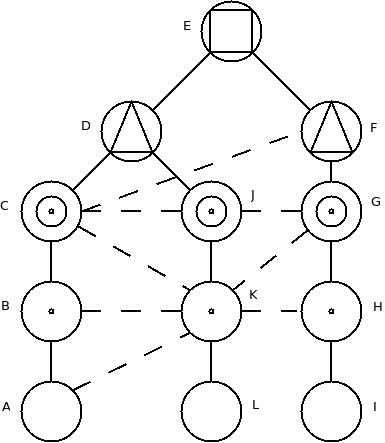
\includegraphics[width=0.5\textwidth]{Imagen/ejercicio9tema1.jpg}
\label{}
\end{figure}
\textbf{1.} Indique las rutas entre las siguientes centrales:\\
\begin{center}
\begin{tabular}{c c c c}
A$\to$L & AKL  		& L$\to$A 	& LKA 	\\
 		& ABKL		&			& LKJCBA	\\
 		& ABCKL		&			& LKJDCBA	\\
 		& ABCDJKL	&			& 	\\
A$\to$I & ABCFGHI  	& L$\to$I 	& LKHI 	\\
 		& ABCDEFGHI	&			& LKJGHI	\\
 		& 			&			& LKJDEFGHI	\\
I$\to$L & IHKL  	& 		 	&  	\\
 		& IHGKL		&			& 	\\
 		& IHGFEDJKL	&			& 	\\
\end{tabular}
\end{center}
\textbf{2.} Calcule el tráfico ofrecido y el tráfico cursado en la sección directa JC/CJ y en la sección final CD/DC.\\
\begin{center}
\begin{tabular}{| c | c | c | c | c | c | c | c | c | c | c | c | c |}
\hline
   & A & B  & C  & D  & E  & F  & G & H  & I  & J  & K  & L \\\hline
 A & - & 15 & 15 & 10 & 5  & 5  & 5 & 10 & 2  & 1  & 8  & 2 \\\hline
 B &   & -  & 15 & 10 & 4  & 5  & 5 & 10 & 2  & 1  & 9  & 1 \\\hline
 C &   &    & -  & 10 & 10 & 20 & 5 & 10 & 5  & 1  & 5  & 5 \\\hline
 D &   &    &    & -  & 10 & 10 & 5 & 1  & 1  & 1  & 0  & 1 \\\hline
 E &   &    &    &    & -  & 5  & 5 & 25 & 10 & 5  & 1  & 0 \\\hline
 F &   &    &    &    &    & -  & 5 & 5  & 10 & 5  & 1  & 1 \\\hline
 G &   &    &    &    &    &    & - & 10 & 5  & 10 & 5  & 5 \\\hline
 H &   &    &    &    &    &    &   & -  & 10 & 15 & 5  & 5 \\\hline
 I &   &    &    &    &    &    &   &    & -  & 10 & 5  & 5 \\\hline
 J &   &    &    &    &    &    &   &    &    & -  & 10 & 10 \\\hline
 K &   &    &    &    &    &    &   &    &    &    & -  & 10 \\\hline
\end{tabular}
\end{center}
Empezamos por calcular el tráfico ofrecido en un sentido y luego en el otro.
\begin{gather*}
TO_{CJ}=TO_{CJpropio}+TO_{AJ}+TO_{BJ}=3E\\
TO_{JC}=TO_{JCpropio}+TO_{KCdesb}+TO_{KBdesb}+TO_{KAdesb}+TO_{JA}+TO_{JB}\\
TO_{KC}=TO_{KCpropio}+TO_{LC}=10\\
TO_{KB}=TO_{KBpropio}+TO_{LB}=10\\
TO_{KA}=TO_{KApropio}+TO_{LA}=10\\
TO_{JC}=1+1+1+1+1+1=6\\
TO_{CD}=TO_{CDpropio}+TO_{CFdesb}+TO_{CJdesb}+TO_{CKdesb}+TO_{CE}+TO_{AD}+TO_{AE}+TO_{BD}+TO_{BE}\\
TO_{CF}=TO_{CFpropio}+TO_{CG}+TO_{CH}+TO_{CI}+TO_{BF}+TO_{BG}+TO_{BH}+TO_{BI}+TO_{AF}+TO_{AG}+\\
+TO_{AH}+TO_{AI}=84E\\
TO_{CJ}=3E\\
TO_{CK}=TO_{CKpropio}+TO_{BKdesb}+TO_{CL}\\
TO_{BK}=TO_{BKpropio}+TO_{AKdesb}+TO_{BL}\\
TO_{AK}=TO_{AKpropio}+TO_{AL}=10E\\
TO_{BK}=11E\\
TO_{CK}=11.1E\\
TO_{CD}=10+8.4+0.3+1.11+10+10+5+10+4=58.81E\\
TO_{DC}=TO_{DCpropio}+TO_{FCdesb}+TO_{JCdesb}+TO_{EC}+TO_{DB}+TO_{EB}+TO_{DA}+TO_{EA}\\
TO_{FC}=TO_{FCpropio}+TO_{GC}+TO_{HC}+TO_{IC}+TO_{FB}+TO_{GB}+TO_{HB}+TO_{IB}+TO_{FA}+TO_{GA}+\\
+TO_{HA}+TO_{IA}=84E\\
TO_{JC}=6E\\
TO_{DC}=10+8.4+0.6+10+10+5+10+4=58E
\end{gather*}
Para terminar calcularemos el tráfico cursado en cada uno de los tramos como $TC=TO(1-P_B)$ siendo $P_B$ la probabilidad de bloqueo en las rutas finales y la probabilidad de desbordamiento en las secciones directas.
\begin{gather*}
TC_{CJ}=TO_{CJ}(1-P_D)=2.7E\\
TC_{JC}=TO_{JC}(1-P_D)=5.4E\\
TC_{CD}=TO_{CD}(1-P_B)=58.22E\\
TC_{DC}=TO_{DC}(1-P_B)=57.42E
\end{gather*}
\end{exercise}
\begin{exercise}[10]
Utilice la red de la figura y la tabla adjunta (que es simétrica) para contestar a las siguientes preguntas:\\
NOTA: La probabilidad de pérdidas en ruta final es del 1 \% y la probabilidad de desbordamiento en secciones directas es del 10\% .
\begin{figure}[H]
\centering
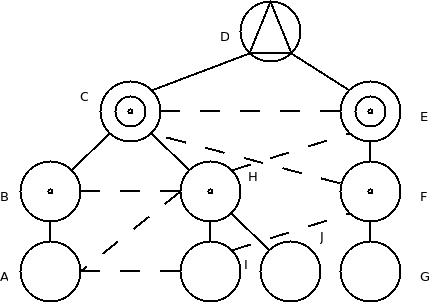
\includegraphics[width=0.5\textwidth]{Imagen/ejercicio10tema1.jpg}
\label{}
\end{figure}
\begin{center}
\begin{tabular}{| c | c | c | c | c | c | c | c | c | c | c |}
\hline
   & A & B  & C  & D  & E  & F  & G & H  & I  & J  \\\hline
 A & - & 15 & 15 & 10 & 3  & 5  & 4 & 10 & 5  & 1  \\\hline
 B &   & -  & 15 & 10 & 3  & 5  & 5 & 10 & 5  & 1  \\\hline
 C &   &    & -  & 10 & 20 & 30 & 1 & 1  & 5  & 2  \\\hline
 D &   &    &    & -  & 10 & 10 & 5 & 1  & 2  & 1  \\\hline
 E &   &    &    &    & -  & 5  & 5 & 25 & 10 & 5  \\\hline
 F &   &    &    &    &    & -  & 5 & 5  & 10 & 2  \\\hline
 G &   &    &    &    &    &    & - & 10 & 5  & 2  \\\hline
 H &   &    &    &    &    &    &   & -  & 5  & 2  \\\hline
 I &   &    &    &    &    &    &   &    & -  & 2  \\\hline
\end{tabular}
\end{center}
\textbf{1.} Rutas entre las siguientes centrales: A$\to$I, I$\to$G, A$\to$G, J$\to$G.\\
\begin{center}
\begin{tabular}{c c c c}
A$\to$I & AI  		& I$\to$G 	& IFG 		\\
 		& ABHI		&			& IHEFG		\\
 		& ABCHI		&			& IHCFG		\\
 		& 			&			& IHCDEFG	\\
A$\to$G & ABCFG  	& J$\to$G 	& JHEFG 	\\
 		& ABCDEFG	&			& JHCFG		\\
 		& 			&			& JHCDEFG	\\
\end{tabular}
\end{center}
\textbf{2.} Tráfico ofrecido y cursado en la sección directa CE/EC.\\
\begin{gather*}
TO_{CE}=TO_{CEpropio}+TO_{HEdesb}+TO_{BE}+TO_{AE}\\
TO_{HE}=TO_{HEpropio}+TO_{IFdesb}+TO_{HF}+TO_{HG}+TO_{JE}+TO_{JF}+TO_{JG}\\
TO_{IF}=TO_{IFpropio}+TO_{IG}=15E\\
TO_{HE}=50.5E\\
TO_{CE}=31.05E\\
TC_{CE}=TO_{CE}(1-P_B)=30.7395E\\
TO_{EC}=TO_{ECpropio}+TO_{FC'desb}+TO_{EB}+TO_{EA}\\
TO_{FC'}=TO_{FCpropio}+TO_{FB}+TO_{FA}+TO_{GC}+TO_{GB}+TO_{GA}=50E\\
TO_{EC}=31E\\
TC_{EC}=30.69E
\end{gather*}
\end{exercise}
\begin{exercise}[11]
En la comunidad Autónoma de Andalucía (con 8 provincia), existe una central secundaria en cada provincia para cursar el tráfico provincial, y solo una central terciaria situada en Sevilla para cursar el tráfico interprovincial. Ahí es precisamente donde se sitúa el proveedor de servicios de Internet o ISP. Asumamos que cada provincia está compuesta por 10 localidades (es un escenario ficticio pero es para poder simplificar el ejercicio), y en cada una de ellas se encuentra situada una central primaria, para cursar el tráfico local. Asimismo, cada localidad está formada por una serie de barrios, y en cada uno de ellos existe una central local con capacidad para 2000 líneas.\\
La arquitectura de la red es la siguiente. Todas las centrales locales bajo la misma central primaria se encuentran conectadas mediante enlaces directos para cursar, en primera instancia, el tráfico local. La probabilidad de desbordamiento en estas secciones directas es del 10\% . Además, cada central local se encuentra conectada a la central secundaria de la que depende jerárquicamente
\end{exercise}